\newpage
\section{Экспериментальная часть}

Проведем тестирование и сравним реализованные алгоритмы по времени.

\subsection{Примеры работ}

Ниже приведены примеры работ при корректных и некорректных данных


\includegraphics[scale=0.35]{zero_arg}

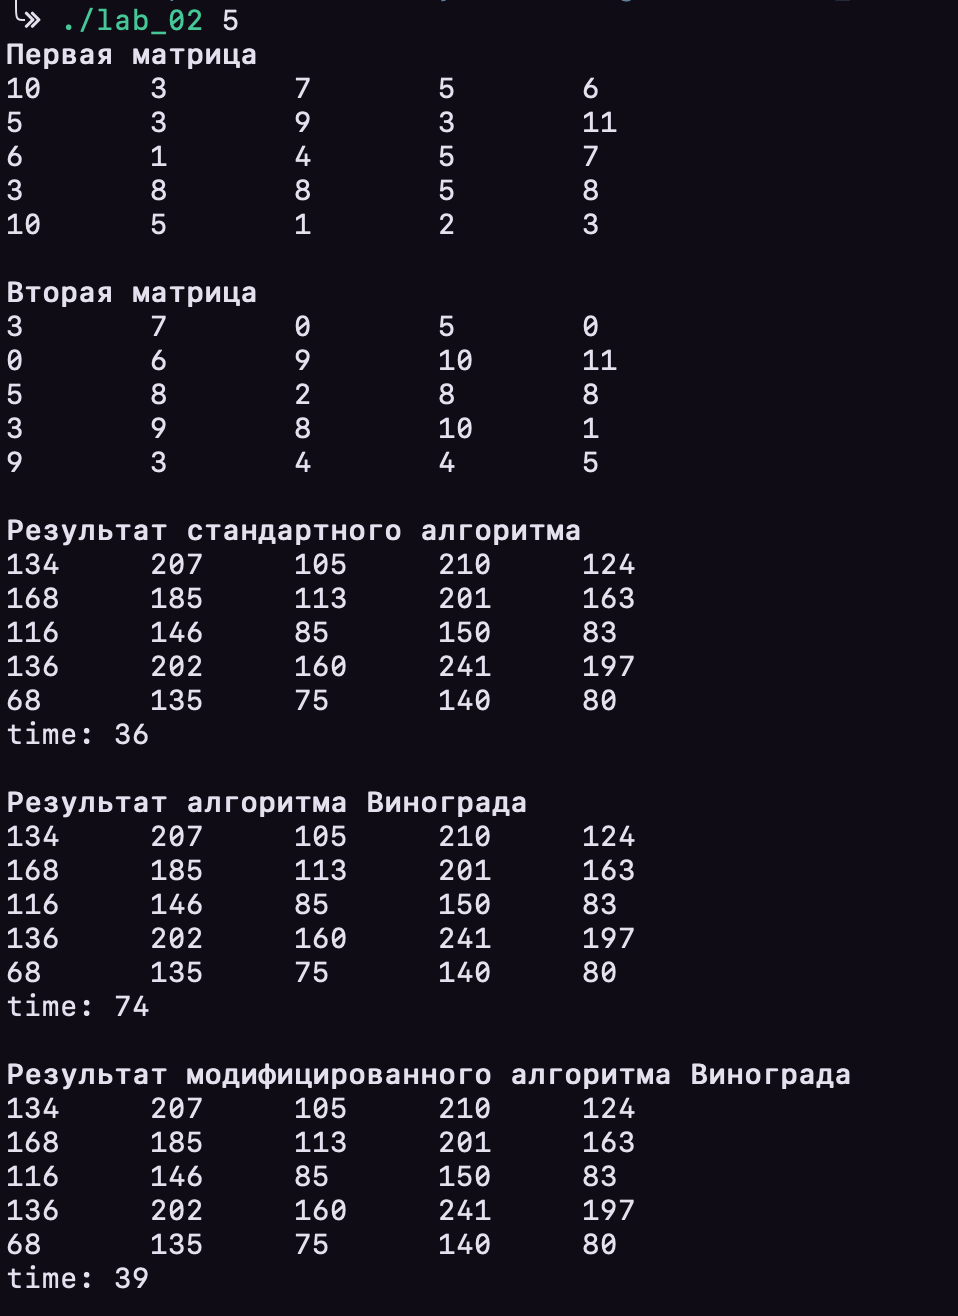
\includegraphics[scale=0.35]{one_arg}

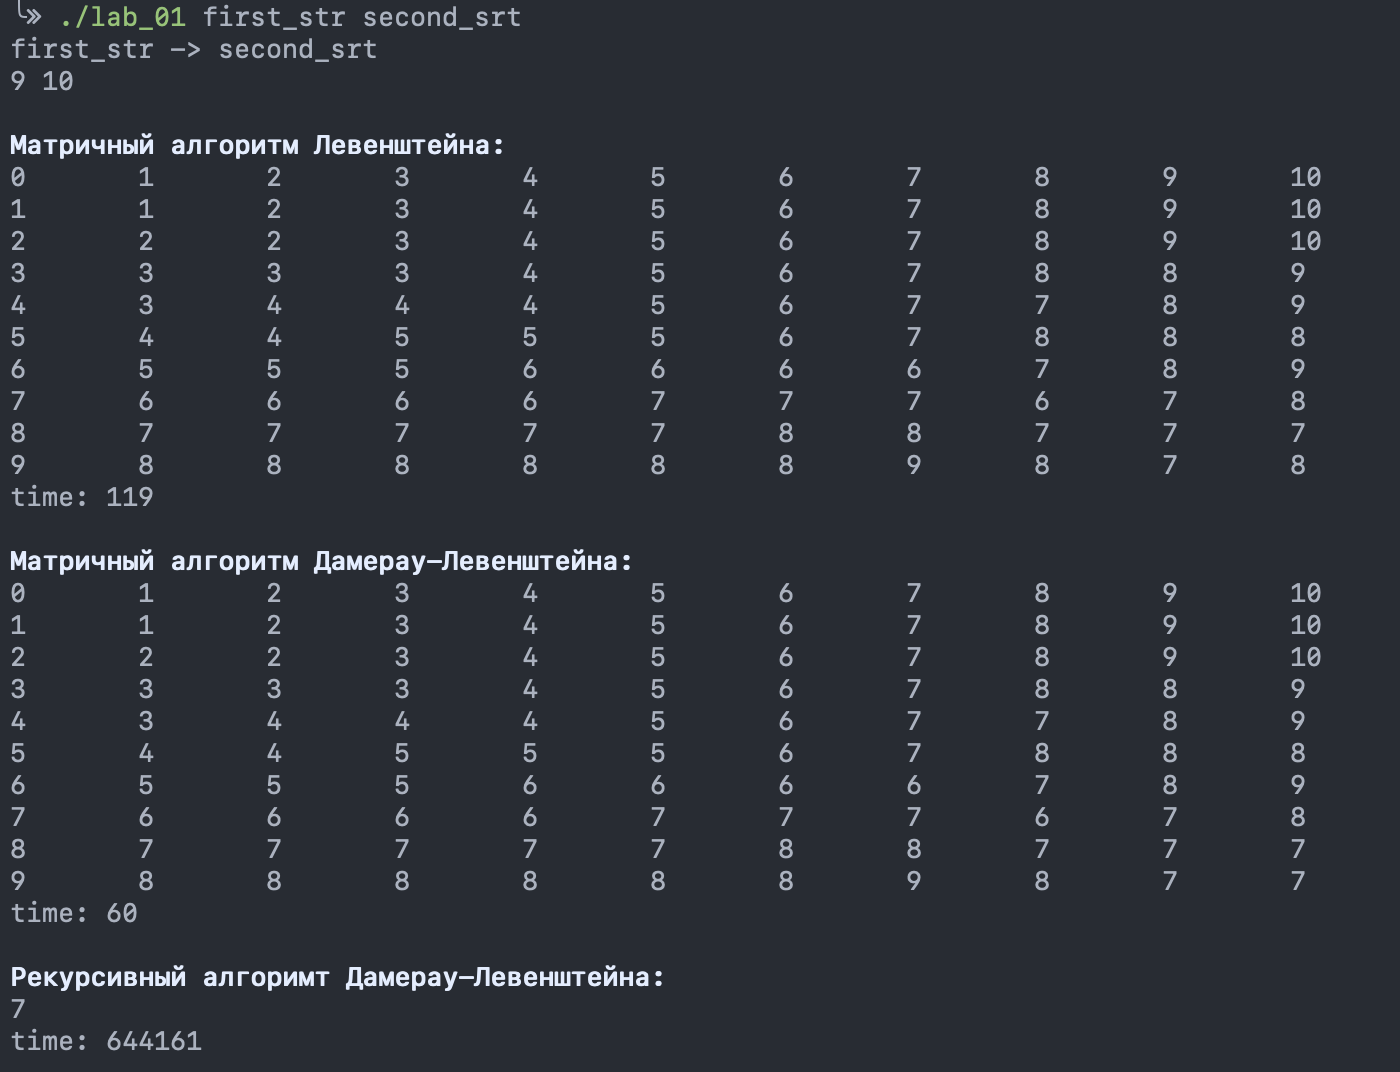
\includegraphics[scale=0.5]{good_work}

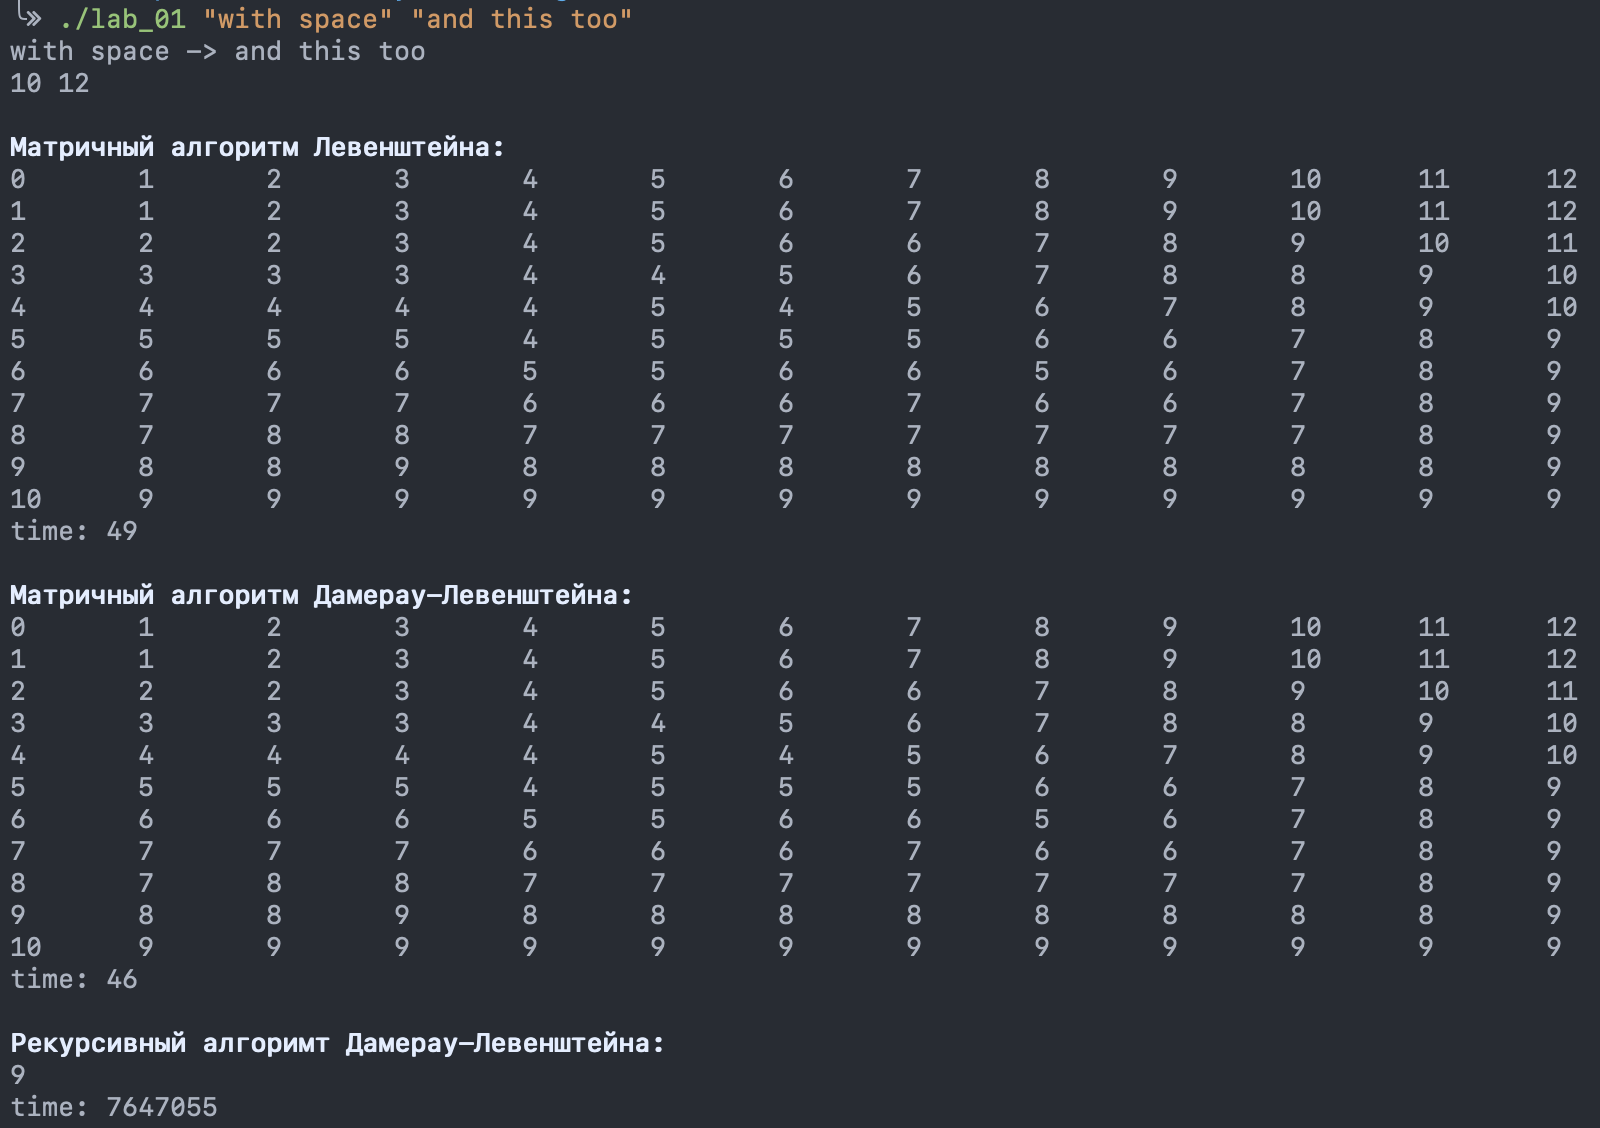
\includegraphics[scale=0.5]{good_space}

\subsection{Результаты тестирования}

Для тестирования были использованы тесты из Таблицы 1 для расстояния
Левенштейна и из Таблицы 2 для расстояния Дамерау-Левенштейна. Ниже
приведены результаты.

\begin{flushright}
    Таблица 3
\end{flushright}

\begin{center}
    Результаты тестирования матричного алгоритма Левенштейна

    \begin{tabular}{|c|c|c|}
        \hline
        $s_1$ & $s_2$ & Результат \\
        \hline
        word & word & 0 \\
        \hline
        word & another & 6 \\
        \hline
        ab & ba & 2 \\
        \hline
        qwerty & qwetry & 2 \\
        \hline
        abcdef & badcfe & 4 \\
        \hline
        werylongword & sh & 12 \\
        \hline
        sh & werylongword & 12 \\
        \hline
        wednesday & weekend & 5 \\
        \hline
        memory & mem & 3 \\
        \hline
        feature & erutaef & 6 \\
        \hline
    \end{tabular}
\end{center}

\hfill

\begin{flushright}
    Таблица 4
\end{flushright}

\begin{center}
    Результаты тестирования матричного алгоритма Дамерау-Левенштейна

    \begin{tabular}{|c|c|c|}
        \hline
        $s_1$ & $s_2$ & Результат \\
        \hline
        word & word & 0 \\
        \hline
        word & another & 6 \\
        \hline
        ab & ba & 1 \\
        \hline
        qwerty & qwetry & 1 \\
        \hline
        abcdef & badcfe & 3 \\
        \hline
        werylongword & sh & 12 \\
        \hline
        sh & werylongword & 12 \\
        \hline
        wednesday & weekend & 5 \\
        \hline
        memory & mem & 3 \\
        \hline
        feature & erutaef & 5 \\
        \hline
    \end{tabular}
\end{center}

\hfill

\begin{flushright}
    Таблица 5
\end{flushright}

\begin{center}
    Результаты тестирования рекурсивного алгоритма Дамерау-Левенштейна

    \begin{tabular}{|c|c|c|}
        \hline
        $s_1$ & $s_2$ & Результат \\
        \hline
        word & word & 0 \\
        \hline
        word & another & 6 \\
        \hline
        ab & ba & 1 \\
        \hline
        qwerty & qwetry & 1 \\
        \hline
        abcdef & badcfe & 3 \\
        \hline
        werylongword & sh & 12 \\
        \hline
        sh & werylongword & 12 \\
        \hline
        wednesday & weekend & 5 \\
        \hline
        memory & mem & 3 \\
        \hline
        feature & erutaef & 5 \\
        \hline
    \end{tabular}
\end{center}

\subsection{Замеры времени}

На рисунках 5 и 6 представлены результаты замера времени алгоритмов на ситуации,
когда размеры строк одинаковы, а на 7 и 8 - когда одна из строк постоянной длины 10.

\begin{tikzpicture}
    \begin{axis}[
        title = Рисунок 5. Две строки одинаковой длины,
        title style = {at={(0.5,-0.2)}},
        legend pos = north west,
        xlabel=Длина строки,
        ylabel=Милисекунды,
        grid = major,
        width = 0.8\paperwidth,
        height = 0.38\paperheight,
        line width = 1
    ]
        \legend{
            Левенштейна матричный,
            Дамерау-Левенштейна матричный
        };
        \addplot[dashed] coordinates {
            (1, 21) (11, 69) (21, 173) (31, 207) (41, 253) (51, 334) (61, 459)
            (71, 586) (81, 733) (91, 894) (101, 1068) (111, 1272) (121, 1582)
            (131, 1793) (141, 1965) (151, 2249) (161, 2519) (171, 2875) (181, 3124)
            (191, 3454) (201, 3824) (211, 4163) (221, 4537) (231, 4947) (241, 5350)
            (251, 5846) (261, 6273) (271, 6714) (281, 7197)(291, 7692) (301, 8200)
            (311, 8732) (321, 9294) (331, 9910) (341, 10423) (351, 11053)
            (361, 11712) (371, 12255) (381, 12946) (391, 14380) (401, 14273)
            (411, 14967) (421, 16551) (431, 16462) (441, 17834) (451, 17905)
            (461, 18692) (471, 19508) (481, 20398) (491, 21116) (501, 21935)
            (511, 22856) (521, 23759) (531, 25452) (541, 25560) (551, 26465)
            (561, 27462) (571, 28427) (581, 29354) (591, 30364) (601, 32142)
            (611, 32342) (621, 33412)(631, 34488) (641, 35643) (651, 37557)
            (661, 37815) (671, 38913) (681, 40069) (691, 41210) (701, 43297)
            (711, 43662) (721, 44888) (731, 46020) (741, 48071) (751, 48514)
            (761, 50870) (771, 51908) (781, 52428) (791, 53698) (801, 56195)
            (811, 56428) (821, 58004) (831, 60044) (841, 60716) (851, 62074)
            (861, 64387) (871, 65186) (881, 66467) (891, 68890) (901, 69687)
            (911, 71000) (921, 73384) (931, 74307) (941, 75929) (951, 78094)
            (961, 78907) (971, 81691) (981, 82229) (991, 84874) (1001, 85432)
        };

        \addplot[black] coordinates {
            (1, 38) (11, 128) (21, 139) (31, 228) (41, 344) (51, 518) (61, 666)
            (71, 854) (81, 1069) (91, 1311) (101, 1579) (111, 1868) (121, 2200)
            (131, 2536) (141, 2916) (151, 3295) (161, 3712) (171, 4155) (181, 4623)
            (191, 5138) (201, 5722) (211, 6186) (221, 6769) (231, 7341) (241, 7931)
            (251, 9433) (261, 9270) (271, 9968) (281, 10683) (291, 11447)
            (301, 12186) (311, 12965) (321, 13799) (331, 14616) (341, 15496)
            (351, 16361) (361, 17295) (371, 18243) (381, 19280) (391, 21172)
            (401, 21229) (411, 22291) (421, 23314) (431, 24364) (441, 25528)
            (451, 26652) (461, 27790) (471, 29738) (481, 30228) (491, 31511)
            (501, 32721) (511, 34028) (521, 35319) (531, 37485) (541, 38017)
            (551, 39406) (561, 40880) (571, 42423) (581, 44504) (591, 45211)
            (601, 46674) (611, 48256) (621, 50721) (631, 51399) (641, 53054)
            (651, 54595) (661, 57060) (671, 57967) (681, 59664) (691, 62451)
            (701, 63143) (711, 66155) (721, 67608) (731, 68549) (741, 71177)
            (751, 72301) (761, 74290) (771, 76833) (781, 77971) (791, 80081)
            (801, 83015) (811, 84006) (821, 86975) (831, 90937) (841, 95018)
            (851, 104317) (861, 101147) (871, 98193) (881, 100037) (891, 103757)
            (901, 103782) (911, 106270) (921, 109067) (931, 111496) (941, 112822)
            (951, 115654) (961, 118642) (971, 120473) (981, 123186) (991, 126838)
            (1001, 127906)
        };
    \end{axis}
\end{tikzpicture}

\begin{tikzpicture}
    \begin{axis}[
        title = Рисунок 6. Две строки одинаковой длины,
        title style = {at={(0.5,-0.2)}},
        legend pos = north west,
        xlabel=Длина строки,
        ylabel=Милисекунды,
        grid = major,
        width = 0.8\paperwidth,
        height = 0.38\paperheight,
        line width = 1
    ]
        \legend{
            Дамерау-Левенштейна матричный,
            Дамерау-Левенштейна рекурсивный
        };
        \addplot[black] coordinates {
            (1, 11) (2, 14) (3, 16) (4, 24) (5, 26) (6, 29) (7, 34) (8, 46) (9, 46)
                        };
        \addplot[dotted] coordinates {
            (1, 3) (2, 10) (3, 22) (4, 183) (5, 338) (6, 2218) (7, 9417) (9, 56574)

        };
    \end{axis}
\end{tikzpicture}

\begin{tikzpicture}
    \begin{axis}[
        title = Рисунок 7. Одна строка длины 10 вторая - переменной длины,
        title style = {at={(0.5,-0.2)}},
        legend pos = north west,
        xlabel=Длина строки,
        ylabel=Милисекунды,
        grid = major,
        width = 0.8\paperwidth,
        height = 0.38\paperheight,
        line width = 1
    ]
        \legend{
            Левенштейна матричный,
            Дамерау-Левенштейна матричный
        };
        \addplot[dashed] coordinates {
            (1, 17) (11, 34) (21, 43) (31, 61) (41, 70) (51, 82) (61, 102)
            (71, 115) (81, 125) (91, 158) (101, 149) (111, 161) (121, 184)
            (131, 196) (141, 209) (151, 220) (161, 239) (171, 244) (181, 259)
            (191, 306) (201, 281) (211, 292) (221, 305) (231, 316) (241, 328)
            (251, 363) (261, 374) (271, 386) (281, 398) (291, 413) (301, 422)
            (311, 435) (321, 448) (331, 459) (341, 471) (351, 484) (361, 498)
            (371, 507) (381, 524) (391, 533) (401, 545) (411, 559) (421, 573)
            (431, 581) (441, 593) (451, 605) (461, 618) (471, 629) (481, 642)
            (491, 654) (501, 666) (511, 721) (521, 733) (531, 745) (541, 759)
            (551, 772) (561, 781) (571, 794) (581, 805) (591, 818) (601, 830)
            (611, 845) (621, 886) (631, 867) (641, 890) (651, 890) (661, 903)
            (671, 915) (681, 926) (691, 939) (701, 954) (711, 963) (721, 975)
            (731, 989) (741, 1000) (751, 1010) (761, 1025) (771, 1036)
            (781, 1127) (791, 1199) (801, 1076) (811, 1085) (821, 1096)
            (831, 1109) (841, 1121) (851, 1156) (861, 1158) (871, 1158)
            (881, 1167) (891, 1182) (901, 1192) (911, 1207) (921, 1217)
            (931, 1229) (941, 1243) (951, 1268) (961, 1267) (971, 1277)
            (981, 1289) (991, 1317) (1001, 1314)
        };

        \addplot[black] coordinates {
            (1, 36) (11, 43) (21, 56) (31, 77) (41, 96) (51, 114) (61, 132)
            (71, 150) (81, 165) (91, 182) (101, 198) (111, 214) (121, 241)
            (131, 259) (141, 275) (151, 291) (161, 308) (171, 325) (181, 341)
            (191, 357) (201, 374) (211, 391) (221, 407) (231, 424) (241, 440)
            (251, 478) (261, 495) (271, 514) (281, 527) (291, 544) (301, 561)
            (311, 577) (321, 595) (331, 612) (341, 627) (351, 644) (361, 660)
            (371, 679) (381, 694) (391, 709) (401, 727) (411, 742) (421, 759)
            (431, 776) (441, 833) (451, 998) (461, 843) (471, 843) (481, 859)
            (491, 876) (501, 892) (511, 953) (521, 969) (531, 984) (541, 1001)
            (551, 1024) (561, 1038) (571, 1055) (581, 1069) (591, 1106)
            (601, 1101) (611, 1115) (621, 1135) (631, 1151) (641, 1168)
            (651, 1187) (661, 1200) (671, 1217) (681, 1234) (691, 1253)
            (701, 1277) (711, 1286) (721, 1301) (731, 1320) (741, 1339)
            (751, 1346) (761, 1364) (771, 1400) (781, 1397) (791, 1415)
            (801, 1430) (811, 1447) (821, 1463) (831, 1480) (841, 1499)
            (851, 1743) (861, 1530) (871, 1549) (881, 1563) (891, 1579)
            (901, 1596) (911, 1611) (921, 1627) (931, 1646) (941, 1664)
            (951, 1678) (961, 1695) (971, 1710) (981, 1727) (991, 1746)
            (1001, 1765)
        };
    \end{axis}
\end{tikzpicture}

\begin{tikzpicture}
    \begin{axis}[
        title = Рисунок 8. Одна строка длины 10 вторая - переменной длины,
        title style = {at={(0.5,-0.2)}},
        legend pos = north west,
        xlabel=Длина строки,
        ylabel=Милисекунды,
        grid = major,
        width = 0.8\paperwidth,
        height = 0.38\paperheight,
        line width = 1
    ]
        \legend{
            Дамерау-Левенштейна матричный,
            Дамерау-Левенштейна рекурсивный
        };
        \addplot[black] coordinates {
            (1, 32) (2, 14) (3, 18) (4, 32) (5, 107) (6, 58) (7, 41) (8, 43) (9, 99)
        };

        \addplot[dotted] coordinates {
            (1, 19) (2, 65) (3, 474) (4, 2537) (5, 11512) (6, 36962) (7, 107236) (8, 355532) (9, 902894)
        };
    \end{axis}
\end{tikzpicture}

\subsection{Выводы}

Из графиков отношения времени к длинам строк видно, что рекурсивный
алгоритм сильно проигрывает матричным. Поэтому выгонее использовать
матричные алгоритмы. Также видно, что алгоритм Дамерау-Левенштейна на 25\%
проигрывает обычному алгоритму Левенштейна на строках длины больше 400.
